\section{Mirabilandia as a micro-city}\label{sec:mira-microcity}

As mentioned in the previous section, Mirabilandia does not offer a recommendation or virtual queuing services.
In this section, we describe a possible implementation of the "smart micro-city" concept applied to the context of amusement parks, specifically that
of Mirabilandia.

\begin{figure}[H]
	\centering
	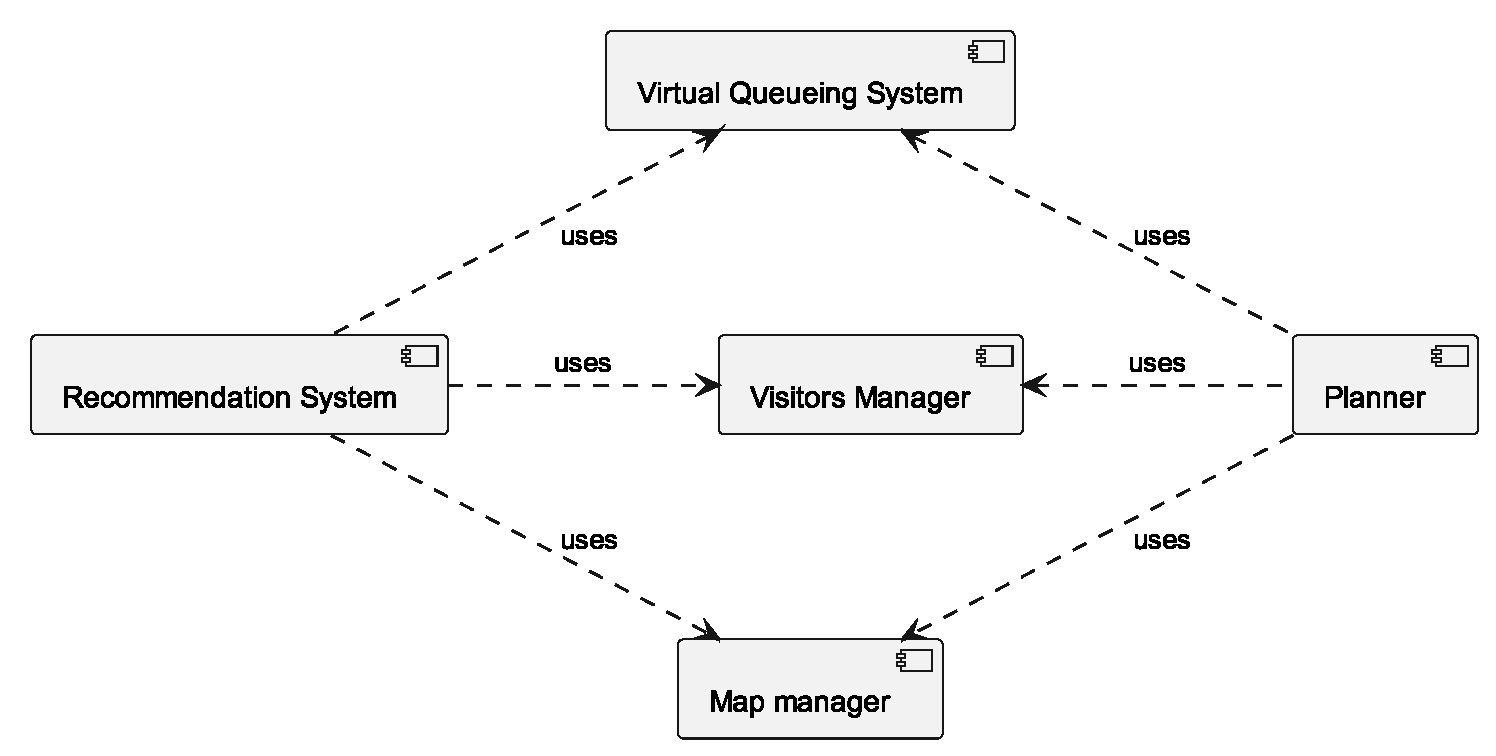
\includegraphics[width=0.6\textwidth]{img/architecture-overview.eps}
	\caption{Overview architecture of Mirabilandia as a micro-city.
		The component diagram shows the rough architecture in the context of Mirabilandia, showing the main dependencies between them.
	}
	\label{fig:architecture-overview}
\end{figure}

Following the analysis of the ``as-is'' system and the goals set to adapt the smart micro-city concept on Mirabilandia,
figure~\ref{fig:architecture-overview} shows the component diagram modeling the entities involved and the main relationships between them.

The main components of the system are the following:

\begin{itemize}
	\item \textit{Map Manager}: is responsible for tracking the guest within the park and providing information about the current position
	\item \textit{Virtual Queueing System}: is responsible for managing the virtual queue for each attraction
	\item \textit{Recommender}: is responsible for providing recommendations to the guests based on their preferences and position within the park
	\item \textit{Planner}: is responsible for planning the itinerary of the guests based on their preferences and crowding of rides
\end{itemize}

From the diagram emerge that \textit{Map Manager} and \textit{Virtual Queueing System} are the main components of the system since they are the ones
that provide information to the other components. The \textit{Map Manager} provides information about the current position of the guests
to the \textit{Recommender} which uses this information to provide recommendations to the guests. Moreover, gives information also to the
\textit{Planner} to avoid crowd situations and maintain a uniform distribution of guests in the park. The \textit{Virtual Queueing System} is used by
the \textit{Planner} to plan the itinerary of the guests and adapt it to reduce the waiting time and improve the quality of the visit within the park
and by the \textit{Recommender} to fetch information about the current waiting time of the attractions and opportunistically advise the attraction.

\subsection{Map Manager}

The location of guests within the amusement park is critical for several reasons: guest location information is used to make recommendations and to determine the best plan for each guest. So, good tracking is crucial for the good working of the overall system.

\begin{figure}[H]
	\centering
	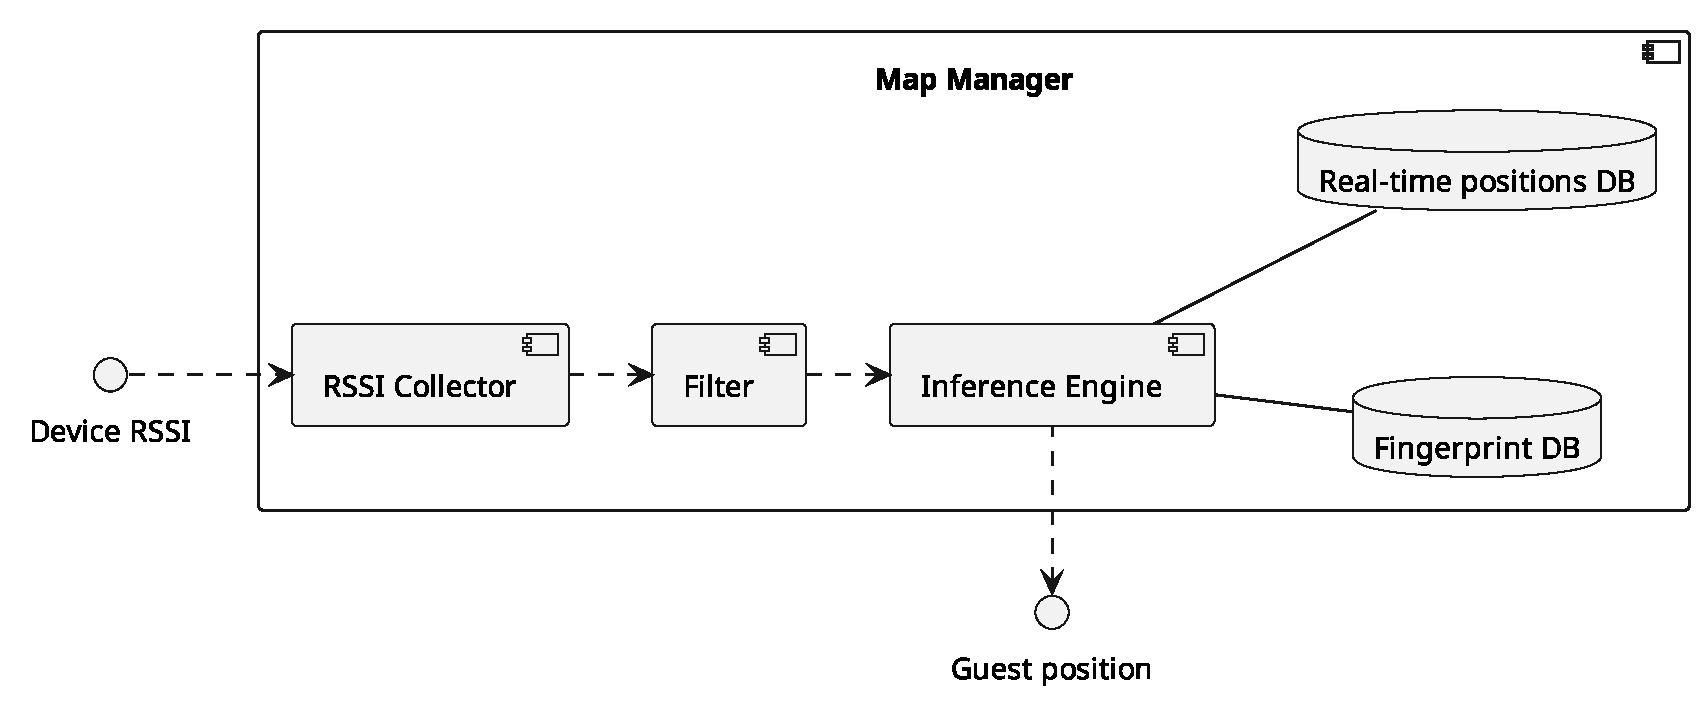
\includegraphics[width=\textwidth]{img/map-manager.eps}
	\caption{Component diagram showing the internal architecture of the \textit{Map Manager} component.
	}
	\label{fig:map-manager}
\end{figure}

\subsection{Virtual Queuing System}

\subsection{Recommender}

\subsection{Planner}
